\documentclass[a4paper,twoside,master.tex]{subfiles}
\begin{document}
\lecture{20}{Friday, February 28, 2020}{Stability Conditions}

\section{Stability Conditions}
\label{sec:stability_conditions}

In our previous lectures, we found properties of systems called extremum conditions. We used the maximization of entropy to show that energy is minimized if entropy is kept constant. By adding temperature and pressure reservoirs, we can translate these conditions to the other thermodynamic potentials to show that they are also minimized when those reservoirs are kept constant.\par

Now we want to find out what makes a system stable. In our previous example with a piston being released, we know that if the piston is in equilibrium, the total energy of the system is at a minimum. If we wiggle the piston away from that minimum, the energy must increase. Let's say that the left compartment has variables $ \{U,S,V,N\} $ and the right compartment has $ \{\tilde{U}, \tilde{S}, \tilde{V}, \tilde{N}\} $. We can write this variation of the wall as the following:
\begin{equation}
    \Delta U_{\text{tot}} \left[ U(S,V + \Delta V, N) - U(S,V,N) \right] + \left[ \tilde{U}(\tilde{S}, \tilde{V} - \Delta V, \tilde{N}) - \tilde{U}(\tilde{S}, \tilde{V}, \tilde{N}) \right]
\end{equation}

Now let's take the opposite perspective. Consider a system with some $ U(S,V,N) $. ``Clone'' it to get an identical copy. Now we bring these two systems together, and we permit an exchange of $ V $. Since A system should be in equilibrium with itself, such a change in volume of either subsystem must increase the energy. We can write this as
\begin{equation}
    \Delta U_{\text{tot}} \left[ U(S,V + \Delta V, N) - U(S,V,N) \right] + \Delta U_{\text{tot}} \left[ U(S,V - \Delta V, N) - U(S,V,N) \right] \geq 0
\end{equation}
or
\begin{equation}
    0 \leq \frac{U_{\text{tot}}}{(\Delta V)^2} = \frac{U(S,V+ \Delta V, N) - 2 U(S,V,N) + U(S, V - \Delta V, N)}{(\Delta V)^2} \underbrace{\to}_{\Delta V \to 0} \eval{\pdv[2]{U}{V}}_{S,N}
\end{equation}

The energy of a stable system must be a convex function of volume, for fixed $ S $ and $ N $. We know that
\begin{equation}
    \eval{\pdv{U}{V}}_{S,N} = -P
\end{equation}
so
\begin{equation}
    - \eval{\pdv{P}{V}}_{S,N} = \eval{\pdv[2]{U}{V}}_{S,N} \geq 0
\end{equation}
so
\begin{equation}
    \kappa_S = - \frac{1}{V} \eval{\pdv{V}{P}}_{S,N} \geq 0
\end{equation}
Therefore, thermodynamic stability requires the adiabatic compressibility to be positive.

Notice, we could do the same thing with any \textit{extensive} variable for any thermodynamic potential and show that the second derivative will probably be positive if the system is stable. Of course, we couldn't do this with something like temperature (we can't just move temperature from one compartment to the other), but let's look at a few more examples. Let's now exchange $ S $ instead of $ V $. This means that
\begin{equation}
    \eval{\pdv[2]{U}{S}}_{V,N} \geq 0
\end{equation}
What does this imply? Recall that
\begin{equation}
    T = \eval{\pdv{U}{S}}_{V,N} \implies \eval{\pdv{T}{S}}_{V,N} = \eval{\pdv[2]{U}{S}}_{V,N} \geq 0 therefore C_V \geq 0
\end{equation}

How about $ F(T,V,N) $ with an exchange of $ V $? By the same argument, we know that $ \eval{\pdv[2]{F}{V}}_{T,N} \geq 0 $.
\begin{equation}
    -P = \eval{\pdv{F}{V}}_{T,N} \implies - \eval{\pdv{P}{V}}_{T,,N} = \eval{\pdv[2]{F}{V}}_{T,N} \geq 0 \implies \kappa_T \geq 0 
\end{equation}

A final example: Take the enthalpy $ H(S,P,N) $ and exchange $ S $. This implies $ \eval{\pdv[2]{H}{S}}_{P,N} \geq 0 $.
\begin{equation}
    T = \eval{\pdv{H}{S}}_{P,N} \implies \eval{\pdv{T}{S}}_{P,N} = \eval{\pdv[2]{H}{S}}_{P,N} \geq 0 \implies C_P \geq 0
\end{equation}

What about our intensive variables, $ \{T, P, \mu\} $? These always show up after exchanging an extensive variable with its intensive partner via a Legendre transform.
\begin{equation}
    U(S,V,N) \overbrace{\to}_{\text{L.T.}} F(T,V,N)
\end{equation}
For the first function, we know a convexity condition with respect to $ S $. $ F(T) $ must therefore be concave!\ This works with every single intensive variable. The second derivative with respect to $ \{T, P, \mu\} $ must be $ \leq 0 $.

\begin{note}{Conclusion}
    Since all thermodynamic potentials with dimension energy (everything but entropy) come from $ U $, and $ U $ is convex in all its extensive variables, we have the following general result: All thermodynamic potentials with dimension energy are convex in their extensive variables and concave in their intensive variables.
\end{note}

In the next chapter, we will be discussing non-ideal gasses. Why might a gas be non-ideal? The answer is that the particles interact with each other. The most common case is that you have a Hamiltonian like
\begin{equation}
    H = \underbrace{\sum_{i=1}^{N} \frac{\va{p}_i^2}{2m}}_{\text{ideal}} + \sum_{i<j} \Phi(\abs{\va{r}_i - \va{r}_j})
\end{equation}
Of course, in real life, there are more than just pairwise interactions. You can have triplet interactions and so on if you have more than two particles. A typical potential might look like the following figure (\Cref{fig:lec_20_pairwise}):


\begin{figure}[h]
    \centering
    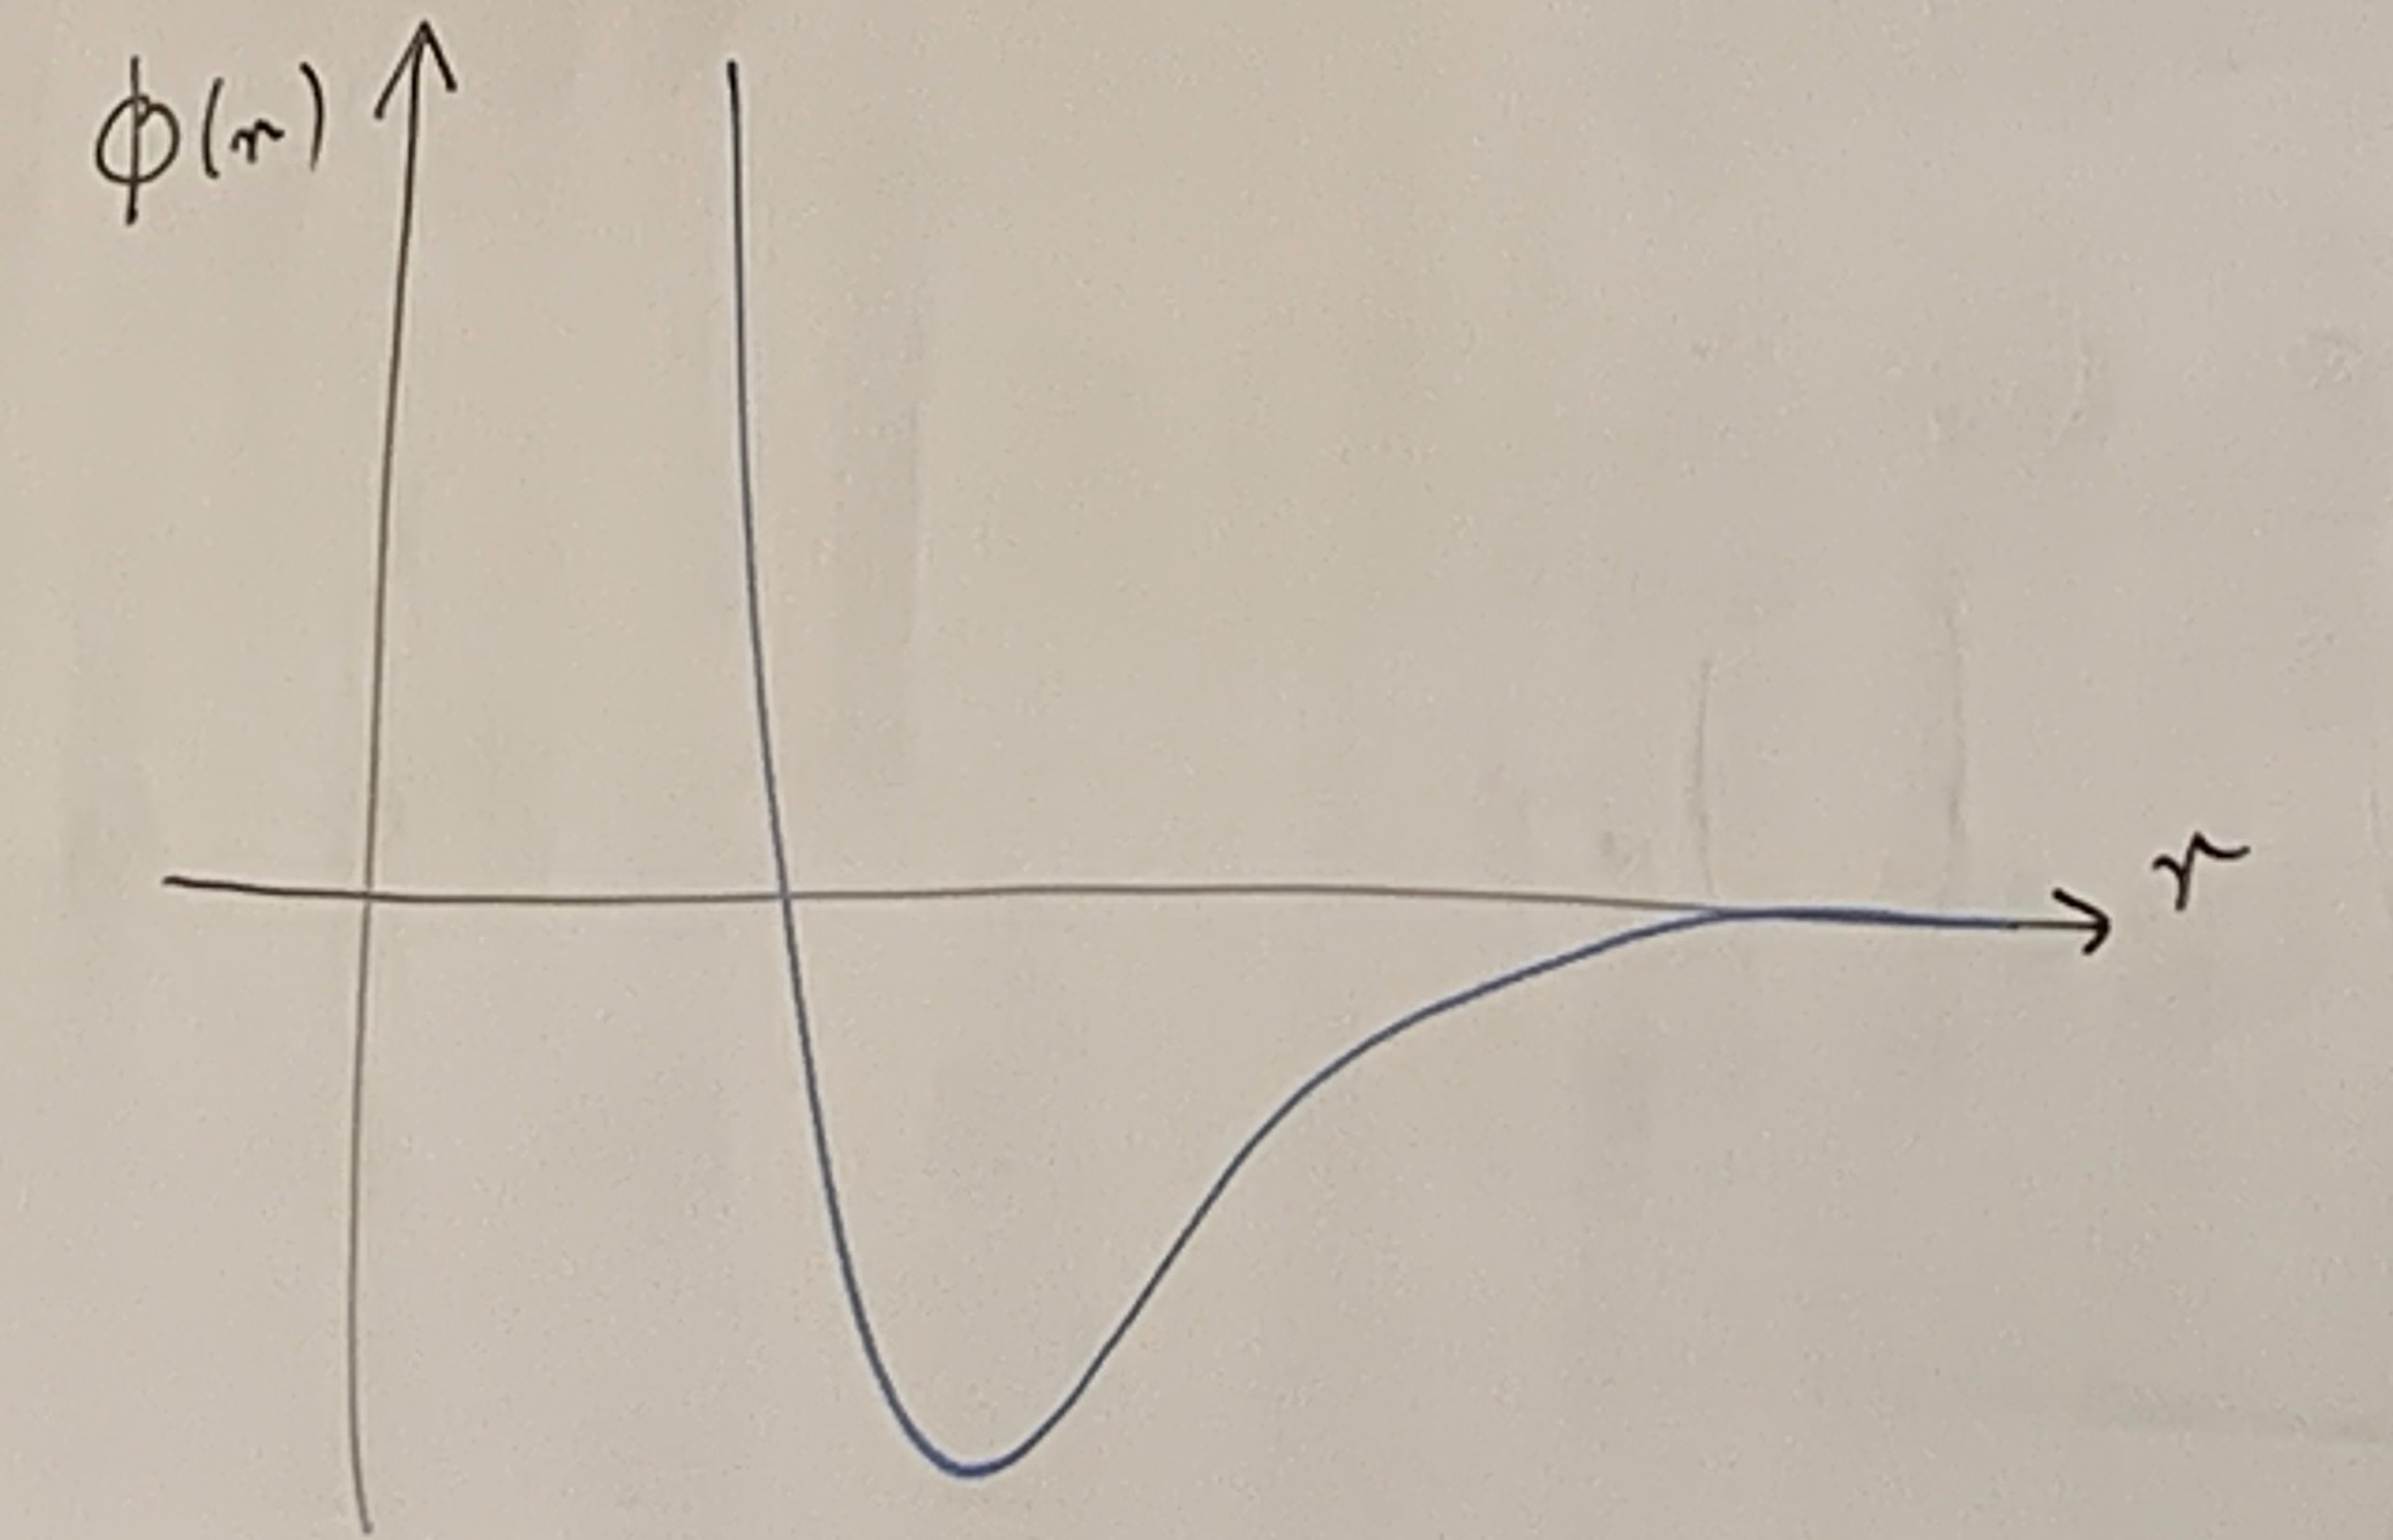
\includegraphics[width=\textwidth]{figures/lec_20_pair_interaction.png}
    \caption{Pairwise Interaction Potential}
    \label{fig:lec_20_pairwise}
\end{figure}





\end{document}
